\documentclass[11pt,tikz]{standalone}
\usepackage[T1]{fontenc}
\usepackage{pgfplots}
\pgfplotsset{compat=1.18}
\begin{document}
	
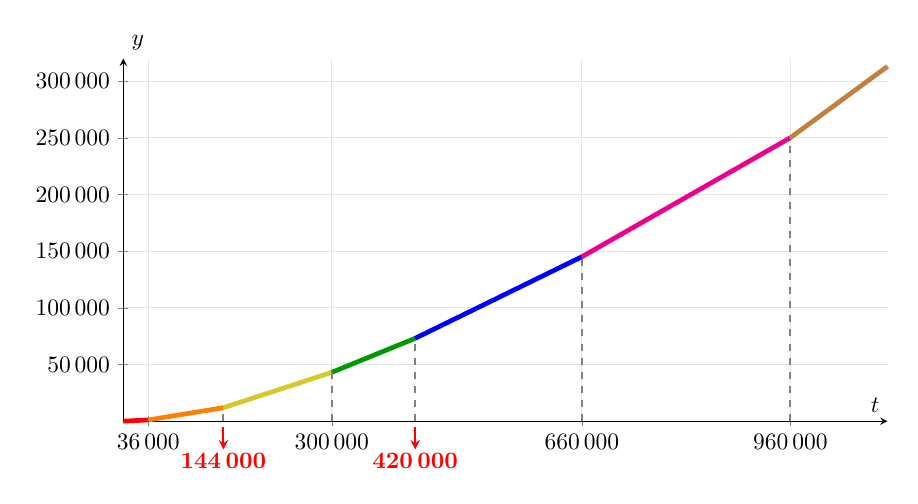
\begin{tikzpicture}[scale=0.85]
	\begin{axis}[
		clip =false,%使文字能显示在图形区域之外
		width=13cm, height=7cm,
		axis lines=middle,
		xlabel=$t$, ylabel=$y$,
		xmin=0, xmax=1100000, ymin=0, ymax=320000,
		scaled ticks=false,
		xtick={0,36000,300000,660000,960000},   
		xticklabels={$O$,36\,000,300\,000,660\,000,960\,000},
		%    extra x ticks={144000,420000},
		%    extra x tick labels={144\,000,420\,000},
		ytick={0,50000,100000,150000,200000,250000,300000},    
%		extra tick style={
%			tick label style={blue,font=\bfseries,yshift=-1em},
%		},
		yticklabels={$O$,50\,000,100\,000,150\,000,200\,000,250\,000,300\,000},
		grid=major, grid style={gray!20},
		ylabel style={above right},
		]
		% 第1段 0-36000: y=0.03t
		\addplot[line width=2pt,red,domain=0:36000,samples=2] {0.03*x} ;
		% 第2段 36000-144000: y=0.1t-2520
		\addplot[line width=2pt,orange,domain=36000:144000,samples=2] {0.1*x-2520};
		% 第3段 144000-300000: y=0.2t-16920
		\addplot[line width=2pt,yellow!80!black,domain=144000:300000,samples=2] {0.2*x-16920};
		% 第4段 300000-420000: y=0.25t-31920
		\addplot[line width=2pt,green!60!black,domain=300000:420000,samples=2] {0.25*x-31920};
		% 第5段 420000-660000: y=0.3t-52920
		\addplot[line width=2pt,blue,domain=420000:660000,samples=2] {0.3*x-52920};
		% 第6段 660000-960000: y=0.35t-85920
		\addplot[line width=2pt,magenta,domain=660000:960000,samples=2] {0.35*x-85920};
		% 第7段 >960000: y=0.45t-181920
		\addplot[line width=2pt,brown,domain=960000:1100000,samples=2] {0.45*x-181920};
		
		% 分段点垂直虚线
		\addplot[dashed,gray,thick,mark=none] coordinates {(36000,0)(36000,1080)};
		\addplot[dashed,gray,thick,mark=none] coordinates {(144000,0)(144000,11880)};
		\addplot[dashed,gray,thick,mark=none] coordinates {(300000,0)(300000,43080)};
		\addplot[dashed,gray,thick,mark=none] coordinates {(420000,0)(420000,73080)};
		\addplot[dashed,gray,thick,mark=none] coordinates {(660000,0)(660000,145080)};
		\addplot[dashed,gray,thick,mark=none] coordinates {(960000,0)(960000,250080)};
		\node[below=10pt,red,font=\bfseries] at (axis cs:144000,0) {144\,000};
		\draw[-stealth,red,thick] (axis cs:144000,-5000) -- (axis cs:144000,-25000);
		
		\node[below=10pt,red,font=\bfseries] at (axis cs:420000,0) {420\,000};
		\draw[-stealth,red,thick] (axis cs:420000,-5000) -- (axis cs:420000,-25000);
	\end{axis}
	
\end{tikzpicture}
\end{document}